\documentclass[t]{beamer}
\usetheme[deutsch]{KIT}
\setbeamercovered{transparent}
\setbeamertemplate{navigation symbols}{}

\KITfoot{Tutoriumsmaterial von Joachim Priesner, Sebastian Ullrich und Max Wagner \hspace{2.5cm} Basierend auf den Folien von Simon Stroh und Moritz v. Looz}
\usepackage[utf8]{inputenc}
\usepackage{amsmath}
\usepackage{ifthen}
\usepackage{amssymb}
\usepackage{tikz}
\usepackage{ngerman}
\usetikzlibrary{automata}
\usenavigationsymbols


\title{Theoretische Grundlagen der Informatik}
\subtitle{Tutorium}
\author{Moritz von Looz, Simon Stroh}

\institute[ITI]{Institut für Theoretische Informatik}

\TitleImage[height=\titleimageht]{images/tmaschine.png}

\newcommand{\N}{\ensuremath{\mathbb{N}}}
\newcommand{\M}{\ensuremath{\mathcal{M}}}
\newcommand{\classP}{\ensuremath{\mathcal{P}}}
\newcommand{\classNP}{\ensuremath{\mathcal{NP}}}
\newcommand{\co}{\ensuremath{\mathsf{co\text{-}}}}
\newcommand{\pot}{\ensuremath{\mathcal{P}}}
\newcommand{\abs}[1]{\ensuremath{\left\vert #1 \right\vert}}
\newcommand{\menge}[2]{\ensuremath{\left\lbrace #1 \,\middle\vert\, #2 \right\rbrace}}
\newcommand{\ducttape}[1]{\vspace{#1}}
\newcommand{\neglit}[1]{\overline{#1\vphantom{x^a}}}
\newcommand{\recipe}{\raisebox{-.3cm}{
\includegraphics[scale=.15]{images/chefs-cap.png}}\hspace{0.2cm}}

\newcommand{\invincible}{\setbeamercovered{invisible}} %  "Yesss! I am invincible!!" (Boris Grishenko)
\newcommand{\vincible}{\setbeamercovered{transparent}}

% \@ifundefined{tikzset}{}{\tikzset{initial text=}} % Text "start" bei Startknoten unterdrücken
\tikzstyle{every node}=[thick]
\tikzstyle{every line}=[thick]

\newcommand{\tutnr}[1]{
  \subtitle{Tutorium #1}
	\begin{frame}
		\maketitle
	\end{frame}
}

\newcommand{\uebnr}[1]{
  \subtitle{Anmerkungen zum #1. Übungsblatt}
	\begin{frame}
		\maketitle
	\end{frame}
}

\begin{document}

\tutnr{10}

\section{Chomsky-Hierarchie}
\subsection*{derp}
\frame{
\frametitle{Grammatiken}
\begin{block}{Definition}
 Eine Grammatik ist ein Regelsystem, mit dem sich die Wörter einer Sprache erzeugen lassen. Sie besteht aus vier Komponenten:
 \begin{itemize}
  \item ein endliches \textbf{Alphabet} $\Sigma$ (auch Terminale genannt)
  \item eine endliche Menge $V$ mit $V \cap \Sigma = \emptyset$ von \textbf{Variablen} (auch Nichtterminale genannt)
  \item ein \textbf{Startsymbol} $S \in V$
  \item eine endliche Menge von \textbf{Ableitungsregeln} $R$ (auch Produktionen genannt).
  Eine Ableitungsregel ist ein Paar ($l,r)$, wobei $l \in (V \cup \Sigma)^+$ und $r \in (V \cup \Sigma)^*$ ist.
  Wir schreiben meist $l \rightarrow r$.
 \end{itemize}
\end{block}
}

\frame{
\frametitle{Beispiel}
\begin{exampleblock}{Beispiel: Sprache der Palindrome}
\begin{align*}
V = &\{S\}\\
\Sigma = &\{0,1\}\\
R = &\{ S \rightarrow \varepsilon \mid 0 \mid 1,\\
       &S \rightarrow 0S0 \mid 1S1 \} 
\end{align*}
\end{exampleblock}
}

\frame{
\frametitle{Chomsky-Hierarchie}
Wir definieren Klassen von Sprachen, die von Grammatiken mit bestimmten Einschränkungen erzeugt werden:
\begin{itemize}
\item CH-3 Regulär/Rechtslinear
\item CH-2 Kontextfrei
\item CH-1 Kontextsensitiv/Längenbeschränkt
\item CH-0 Beliebig (rekursiv aufzählbar)
\end{itemize}
Es gilt: $$CH-3 \subset CH-2 \subset CH-1 \subset CH-0$$
Frage: Welche Sprachen liegen nicht in CH-0 ?
}

\frame{
\frametitle{CH-0}
Rekursiv aufzählbare Sprachen
\begin{itemize}
\item Sprachen, die von einer beliebigen Grammatik erzeugt werden
\item Genau die Sprachen, die DTM \& NTM akzeptieren können
\end{itemize}

}

\frame{
\frametitle{CH-1}
Kontextsensitive/längenbeschränkte Sprachen
\begin{itemize}
\item Sprachen, die von Grammatiken erzeugt werden, deren Ableitungen eine kürzere linke als rechte Seite haben. D.h. Produktionen machen das Wort immer länger.
\item (Genau die Sprachen, die von linear beschränken Turingmaschinen erkannt werden)
\end{itemize}
~\micropause
\begin{block}{Beispiel}
\begin{itemize}
\item Die Programmiersprache C (typedef)
\item Die Sprache der wohlgeformten Latex-Dokumente
\end{itemize}
\end{block}
}

\frame{
\frametitle{CH-2}
Kontextfreie Sprachen
\begin{itemize}
\item Grammatiken, deren Ableitungsregeln auf der linken Seite immer aus genau einem Nichtterminalsymbol bestehen
\item Genau die Sprachen, die von Kellerautomaten erkannt werden (Vorgriff)
\end{itemize}
~\micropause
\begin{block}{Beispiele}
\begin{itemize}
\item Lojban
\item Die Sprache der gültigen Klammerausdrücke
\item Die Sprache der regulären Ausdrücke
\end{itemize}
\end{block}
}

\frame{
\frametitle{CH-3}
Reguläre Sprachen
\begin{itemize}
\item Grammatiken, deren Ableitungsregeln ausschließlich die folgende Form haben:
$$A\rightarrow v \mbox{ mit } A \in V \mbox{ und } v = \varepsilon \mbox{ oder } v = aB \mbox{ mit } a \in \Sigma \mbox{,} B \in V$$
\item Genau die Sprachen, die von endlichen Automaten erkannt werden
\end{itemize}
~\micropause
\begin{block}{Beispiele}
\begin{itemize}
\item Alle endlichen Sprachen
\item Tokens ($\rightarrow$ vgl. Compilerbau)
\end{itemize}
\end{block}
}

\begin{frame}
\frametitle{Aufgabe}
Gegeben sei die Grammatik $G = (\Sigma, V, S, R)$ mit $\Sigma = \{a, b\}$,
$V = \{S, A\}$ und 
\[ R = \{S \rightarrow AA, \quad A \rightarrow AAA,
\quad A \rightarrow bA, \quad A \rightarrow Ab, \quad A \rightarrow a\}. \]

\begin{itemize}
  \item Welchen Typ in der Chomsky-Hierarchie hat $G$?

  \item Welche Zeichenketten aus $\Sigma^*$ k\"onnen in vier Schritten abgeleitet werden?

  \item Sei $\alpha = (b^*ab^*ab^*)^+$ ein regul\"arer Ausdruck.
        Zeige: $L(\alpha) \subseteq L(G)$.
\end{itemize}
\end{frame}


\begin{frame}
\frametitle{Aufgabe: CH-1-Grammatiken}
Konstruiere eine Typ-1-Grammatik, welche die Sprache

\begin{quote}
  $L = \{a^n b^n c^n \, | \, n \geq 1\}$
\end{quote}

erzeugt.


\pause
\begin{block}{Lösung}
\begin{align*}
&\Sigma = \{a, b, c\} \\
&V = \{ S, \# \} \\
&S \rightarrow aS\#c \mid abc \\
&c\# \rightarrow \#c \\
&b\# \rightarrow bb
\end{align*}
\end{block}
\end{frame}

\begin{frame}
\frametitle{Aufgabe: CH-2-Grammatiken}
Gib eine kontextfreie Grammatik an, die die Sprache
\begin{quote}
  $L = \{w \in \Sigma^* \, | \, w \text{ enth\"alt mehr Nullen als Einsen}\}$  
\end{quote}
\"uber dem Alphabet $\Sigma = \{0, 1\}$ beschreibt.


\pause
\begin{block}{Lösung}
\begin{align*}
S &\rightarrow 0S1S' \mid 0S'1S \mid 1S0S' \mid 1S'0S \mid 0 \\
S' &\rightarrow 0 \mid \varepsilon
\end{align*}
\end{block}
\end{frame}


\begin{frame}
\frametitle{Aufgabe: CH-3-Grammatiken}
Gib unter Anwendung des Verfahrens aus Satz 5.5 eine Grammatik an,
welche genau die Sprache erzeugt, die folgender DEA akzeptiert:

\begin{center}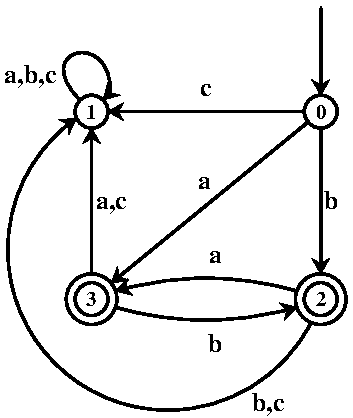
\includegraphics[scale=0.8]{./images/dea1.pdf}\end{center}
\end{frame}


\begin{frame}
\begin{enumerate}
\item Bestimme eine möglichst kurze Grammatik $G_R$ für reguläre Ausdrücke über dem Alphabet $\Sigma = \{0,1\}$ mit maximalem Chomsky-Typ.
\item Bestimme einen Ableitungsbaum für das Wort $1^* \cup (01)^*$. 
\item Ist die Grammatik eindeutig? Diskutiere, ob es eine eindeutige Grammatik für reguläre Ausdrücke geben kann, falls die angegebene Grammatik mehrdeutig ist.
\end{enumerate}
\end{frame}

\frame{
\frametitle{Probleme}
Es gibt einige interessante Probleme, mit deren Entscheidbarkeit, Komplexität bzw. Abgeschlossenheit wir uns noch befassen (jeweils für die Klassen)
\begin{itemize}
\item Das Wortproblem
\item Vereinigung
\item Schnitt
\item Komplement
\item Konkatenation
\item Kleenescher Abschluss (*-Operator)
\end{itemize}
}

\frame{
  \frametitle{Lizenzen}
  \center
  \includegraphics[width=2em]{images/by}
  \includegraphics[width=2em]{images/cc}
  \includegraphics[width=2em]{images/sa}
  \\
  {\tiny

Dieses Werk ist unter einem ``Creative Commons Namensnennung-Weitergabe unter gleichen Bedingungen 3.0 Deutschland``-Lizenzvertrag lizenziert. Um eine Kopie der Lizenz zu erhalten, gehen Sie bitte zu \href{http://creativecommons.org/licenses/by-sa/3.0/de/}{http://creativecommons.org/licenses/by-sa/3.0/de/} oder schreiben Sie an Creative Commons, 171 Second Street, Suite 300, San Francisco, California 94105, USA.\\
  \vspace{1cm}
  Davon ausgenommen sind das Titelbild, welches aus der März-April 2002 Ausgabe von American Scientist erschienen ist und ohne Erlaubnis verwendet wird, sowie das KIT Beamer Theme. Hierfür gelten die Bestimmungen der jeweiligen Urheber.
  \vspace{1cm}
  \\ 
  }
  %Habe hier die Reihenfolge etwas umgestellt, weil die Formatierung bei mir komisch aussah. 
  %Wenn es bei dir anders ist, kannst du es auch wieder zurückändern, dann haben wir unterschiedliche Kompilieroptionen
}

\end{document}
